\documentclass{article}
\usepackage{graphicx}
\usepackage{amsmath}
\usepackage{amssymb}
\usepackage{listings}
\usepackage[margin=1in]{geometry}
\usepackage{xcolor}
\usepackage{tikz}
\usetikzlibrary{shapes, arrows, positioning, calc}
\usepackage{tcolorbox}
\usepackage{hyperref}

% Define colors for syntax highlighting
\definecolor{codegreen}{rgb}{0,0.6,0}
\definecolor{codegray}{rgb}{0.5,0.5,0.5}
\definecolor{codepurple}{rgb}{0.58,0,0.82}
\definecolor{backcolour}{rgb}{0.95,0.95,0.92}

% Python style for highlighting
\lstdefinestyle{pythonstyle}{
    backgroundcolor=\color{backcolour},   
    commentstyle=\color{codegreen},
    keywordstyle=\color{magenta},
    numberstyle=\tiny\color{codegray},
    stringstyle=\color{codepurple},
    basicstyle=\ttfamily\footnotesize,
    breakatwhitespace=false,         
    breaklines=true,                 
    captionpos=b,                    
    keepspaces=true,                 
    numbers=left,                    
    numbersep=5pt,                  
    showspaces=false,                
    showstringspaces=false,
    showtabs=false,                  
    tabsize=2
}
\lstset{style=pythonstyle}

\title{Lecture: Building Modern CNNs\\Practical Scaling \& the Modern CNN Era}
\author{Deep Learning Class}
\date{\today}

\begin{document}
\maketitle

\tableofcontents
\newpage

\section{Introduction: A Tale of Two Paradigms}

\subsection{Setting the Stage: The Post-ResNet Era and the ViT Disruption}

The late 2010s computer vision landscape was dominated by CNNs. Architectures like ResNet, DenseNet, and Inception established a paradigm centered on clever connectivity patterns, depth, and multi-scale feature extraction. The core assumption---that spatial locality and translation equivariance inherent in convolution are fundamental inductive biases for images---was rarely questioned.

This paradigm faced disruption in 2020 with Vision Transformers (ViTs). By adapting the Transformer architecture from NLP to vision, researchers demonstrated that pure self-attention mechanisms could outperform leading CNNs. However, this came with a caveat: ViTs required pre-training on massive datasets to overcome their lack of built-in image-specific biases. The ViT's success ignited a fundamental debate: strong, hard-coded CNN priors versus flexible, data-driven Transformer learning.

\subsection{The Central Questions}

This lecture addresses two pivotal questions:

\begin{enumerate}
    \item \textbf{Intelligent Scaling:} If we have larger computational budgets, how do we spend them wisely to maximize accuracy? This moves beyond efficiency to principled model growth (EfficientNet).
    
    \item \textbf{Architectural Relevance:} Was the CNN architecture fundamentally limited, or were training recipes and micro-designs simply outdated? (ConvNeXt hypothesis)
\end{enumerate}

\begin{tcolorbox}[colback=yellow!5!white, colframe=orange!50!black, title=The Deeper Truth]
State-of-the-art performance is not a product of architecture alone. It emerges from the tight coupling of network architecture, training recipe, and data augmentation strategy. ConvNeXt demonstrated this by closing the performance gap with ViTs through recipe modernization \textit{before} any architectural changes.
\end{tcolorbox}

\subsection{Lecture Roadmap}

\begin{itemize}
    \item \textbf{Part I:} The Science of Scaling---compound scaling methodology
    \item \textbf{Part II:} The Great Convergence---modernizing CNN blocks
    \item \textbf{Part III:} The Unseen Engine---modern training recipes
    \item \textbf{Part IV:} From Theory to Practice---enhanced implementations
    \item \textbf{Part V:} The Broader Horizon---hybrid architectures and future directions
\end{itemize}

\section{Part 1: Practical Scaling}

\subsection{The Three Dimensions of Scaling}

When we want to increase model capacity, we have three fundamental ``knobs'' to turn:

\begin{enumerate}
    \item \textbf{Depth ($D$):} Add more layers
    \begin{itemize}
        \item \textit{Benefit:} Richer hierarchical features, larger effective receptive field (ERF)
        \item \textit{Cost:} Harder optimization, vanishing gradients, diminishing returns
    \end{itemize}
    
    \item \textbf{Width ($W$):} Increase channels per layer
    \begin{itemize}
        \item \textit{Benefit:} More capacity to capture fine-grained features
        \item \textit{Cost:} Parameters and FLOPs grow \textit{quadratically} (Conv layer: $\mathcal{O}(C_{in} \times C_{out})$)
    \end{itemize}
    
    \item \textbf{Resolution ($R$):} Use larger input images
    \begin{itemize}
        \item \textit{Benefit:} Capture finer spatial details
        \item \textit{Cost:} Compute and activation memory grow quadratically ($\mathcal{O}(H \times W)$)
    \end{itemize}
\end{enumerate}

\subsection{The Problem with Single-Axis Scaling}

\begin{tcolorbox}[colback=red!5!white, colframe=red!75!black, title=Critical Observation]
Scaling only \textit{one} dimension quickly saturates accuracy while wasting computational budget. A balanced approach is essential.
\end{tcolorbox}

Figure~\ref{fig:efficientnet_scaling} illustrates this phenomenon. When scaling only width, depth, or resolution independently, accuracy improvements plateau rapidly. In contrast, compound scaling maintains consistent gains as the model grows.

\begin{figure}[h]
    \centering
    \includegraphics[width=0.45\linewidth]{Module 4-CNN/fig1_effNet.png}
    \includegraphics[width=0.52\linewidth]{Module 4-CNN/fig2_EfficientNet.png}
    \caption{\textbf{Left:} EfficientNet model family achieves superior accuracy with significantly fewer parameters and FLOPs compared to previous state-of-the-art CNNs. The compound scaling creates models from B0 to B7 that lie on an efficient frontier. \textbf{Right:} Model scaling strategies comparison. Scaling a single dimension (width, depth, or resolution) saturates quickly, while compound scaling maintains efficiency.  (Figures from Tan \& Le, 2019)}
    \label{fig:efficientnet_scaling}
\end{figure}

For example:
\begin{itemize}
    \item Increasing only width without adding depth means the network cannot learn more complex feature hierarchies
    \item Increasing only resolution without more channels means the network cannot capture the additional fine details revealed by larger images
    \item Increasing only depth makes training unstable and hits diminishing returns
\end{itemize}

\textbf{Key insight from Figure~\ref{fig:efficientnet_scaling}:} Notice how the compound scaling curve (yellow) continues to improve while single-axis curves flatten. This validates the interdependence of the three dimensions---they must grow together to effectively utilize increased computational budget.

\subsection{EfficientNet's Compound Scaling: A First-Principles Analysis}

EfficientNet introduced a principled approach: scale all three dimensions simultaneously using a single compound coefficient $\phi$.

\subsubsection{The Scaling Rule}

Given a baseline network (e.g., EfficientNet-B0 with $\phi = 0$), we scale:

\begin{equation}
D = \alpha^\phi, \quad W = \beta^\phi, \quad R = \gamma^\phi
\end{equation}

where $(\alpha, \beta, \gamma)$ are constants determined once via grid search on the baseline, subject to a specific constraint.

\subsubsection{Deriving the FLOP Constraint}

The total FLOPs of a CNN are approximately:
\begin{equation}
\text{FLOPs} \propto D \cdot W^2 \cdot R^2
\end{equation}

\textbf{Why quadratic terms?}
\begin{itemize}
    \item $W^2$: Both input and output channels scale with $W$ in conv layers
    \item $R^2$: Both height and width of feature maps scale with $R$
\end{itemize}

Substituting the scaling rules:
\begin{align}
\text{FLOPs}(\phi) &\propto (\alpha^\phi) \cdot (\beta^\phi)^2 \cdot (\gamma^\phi)^2 \\
&= \alpha^\phi \cdot \beta^{2\phi} \cdot \gamma^{2\phi} \\
&= (\alpha \cdot \beta^2 \cdot \gamma^2)^\phi
\end{align}

To achieve predictable, exponential growth where each $\phi$ increment doubles FLOPs:
\begin{equation}
\alpha \cdot \beta^2 \cdot \gamma^2 \approx 2
\end{equation}

This ensures: $\text{FLOPs}(\phi) \approx 2^\phi \cdot \text{FLOPs}_{\text{baseline}}$

\subsubsection{EfficientNet Constants}

Grid search on EfficientNet-B0 yielded:
\begin{equation}
\alpha \approx 1.2, \quad \beta \approx 1.1, \quad \gamma \approx 1.15
\end{equation}

Verification: $1.2 \times (1.1)^2 \times (1.15)^2 = 1.2 \times 1.21 \times 1.3225 \approx 1.92 \approx 2$ \checkmark

\textbf{Interpretation:}
\begin{itemize}
    \item Depth scales fastest (20\% per $\phi$) --- training stability from residual connections allows this
    \item Width scales slowest (10\% per $\phi$) --- quadratic parameter cost makes aggressive width scaling expensive
    \item Resolution scales moderately (15\% per $\phi$) --- balances detail capture with memory constraints
\end{itemize}

\subsubsection{The Interdependence Argument}

The scaling dimensions are not independent:

\begin{enumerate}
    \item \textbf{$R \uparrow$ without $W \uparrow$:} Network lacks capacity to process fine-grained details from higher resolution
    \item \textbf{$R \uparrow$ without $D \uparrow$:} ERF remains too small to capture global context in larger images
    \item \textbf{$W \uparrow$ or $D \uparrow$ without $R \uparrow$:} Insufficient input information to leverage increased model capacity
\end{enumerate}

\begin{tcolorbox}[colback=blue!5!white, colframe=blue!75!black, title=Design Principle]
Balanced scaling is not optional---it's necessary. Single-axis scaling wastes computational budget by creating capacity-information mismatches.
\end{tcolorbox}

\begin{center}
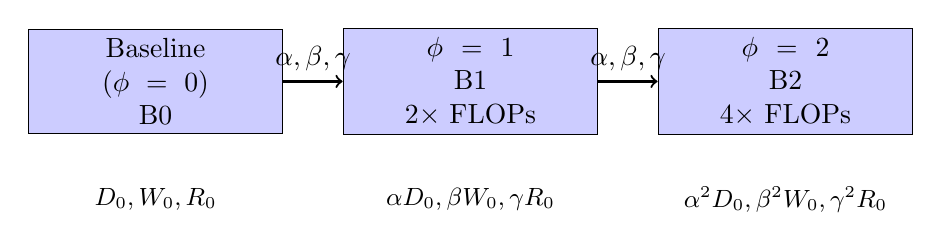
\begin{tikzpicture}[node distance=2cm, auto,
    blockstyle/.style={rectangle, draw, fill=blue!20, text width=3cm, text centered, minimum height=1cm}]
    
    \node[blockstyle] (baseline) {Baseline\\($\phi=0$)\\B0};
    \node[blockstyle, right of=baseline, node distance=4cm] (b1) {$\phi=1$\\B1\\$2\times$ FLOPs};
    \node[blockstyle, right of=b1, node distance=4cm] (b2) {$\phi=2$\\B2\\$4\times$ FLOPs};
    
    \draw[->, thick] (baseline) -- (b1) node[midway, above] {$\alpha, \beta, \gamma$};
    \draw[->, thick] (b1) -- (b2) node[midway, above] {$\alpha, \beta, \gamma$};
    
    \node[below of=baseline, node distance=1.5cm] {\small $D_0, W_0, R_0$};
    \node[below of=b1, node distance=1.5cm] {\small $\alpha D_0, \beta W_0, \gamma R_0$};
    \node[below of=b2, node distance=1.5cm] {\small $\alpha^2 D_0, \beta^2 W_0, \gamma^2 R_0$};
\end{tikzpicture}
\end{center}

\subsection{Practical Guidelines for Scaling}

\begin{tcolorbox}[colback=blue!5!white, colframe=blue!75!black, title=Rules of Thumb]
\begin{itemize}
    \item Start with modest resolution ($160$-$224$)
    \item Increase width until near memory limit
    \item Add depth where residual connections are stable
    \item Avoid combining tiny blocks with huge resolution
    \item If latency-bound on device, prefer width over resolution increases
    \item \textbf{Always verify on target hardware} (FLOPs $\neq$ latency!)
\end{itemize}
\end{tcolorbox}

\section{Part 2: The CNN Renaissance (Post-ViT Era)}

\subsection{The Challenge}

In 2020-2021, Vision Transformers (ViTs) rapidly gained dominance:
\begin{itemize}
    \item Outperformed ResNet and EfficientNet on ImageNet
    \item Demonstrated excellent scaling with massive datasets
    \item Introduced global self-attention mechanism
\end{itemize}

This raised a critical question: Is the CNN architecture fundamentally limited, or were the training recipes and micro-designs (like the ResNet block) simply outdated?

\subsection{ConvNeXt: A ConvNet for the 2020s}

ConvNeXt (2022) systematically modernized ResNet-50 to match ViT performance, demonstrating that CNNs remain highly competitive when properly designed and trained.

\subsubsection{Modernization Roadmap: ResNet-50 $\rightarrow$ ConvNeXt}

\textbf{Step 1: Modern Training Recipe (Major Boost!)}

This alone provided a massive improvement. The ``recipe'' matters as much as the architecture!

\textbf{Step 2: Macro Design Changes}
\begin{itemize}
    \item Adjusted stage compute ratio (allocate more blocks to later stages)
    \item ``Patchify'' stem: Replace ResNet's complex stem (7x7 conv + pool) with a 4x4 non-overlapping convolution (mimicking ViT's patch embedding)
\end{itemize}

\textbf{Step 3: Inverted Bottleneck \& Depthwise Convolutions}

Adopt the MobileNetV2 inverted bottleneck design:
\begin{itemize}
    \item \textit{Traditional bottleneck:} Compress $\rightarrow$ Process $\rightarrow$ Expand
    \item \textit{Inverted bottleneck:} Expand $\rightarrow$ Process (depthwise) $\rightarrow$ Project
\end{itemize}

This is more efficient: spatial processing happens in an expanded dimension where depthwise convolutions are cheap.

\textbf{Step 4: Large Kernel Sizes}

Increase depthwise kernel from 3x3 to 7x7 (mimicking ViT's attention window size and expanding ERF).

\textbf{Step 5: Micro Design Refinements}
\begin{itemize}
    \item Replace ReLU with GELU activation
    \item Replace BatchNorm with LayerNorm
    \item Reduce total number of normalization and activation layers
\end{itemize}

\subsection{Comparing Block Designs}

\begin{figure}[h]
\centering
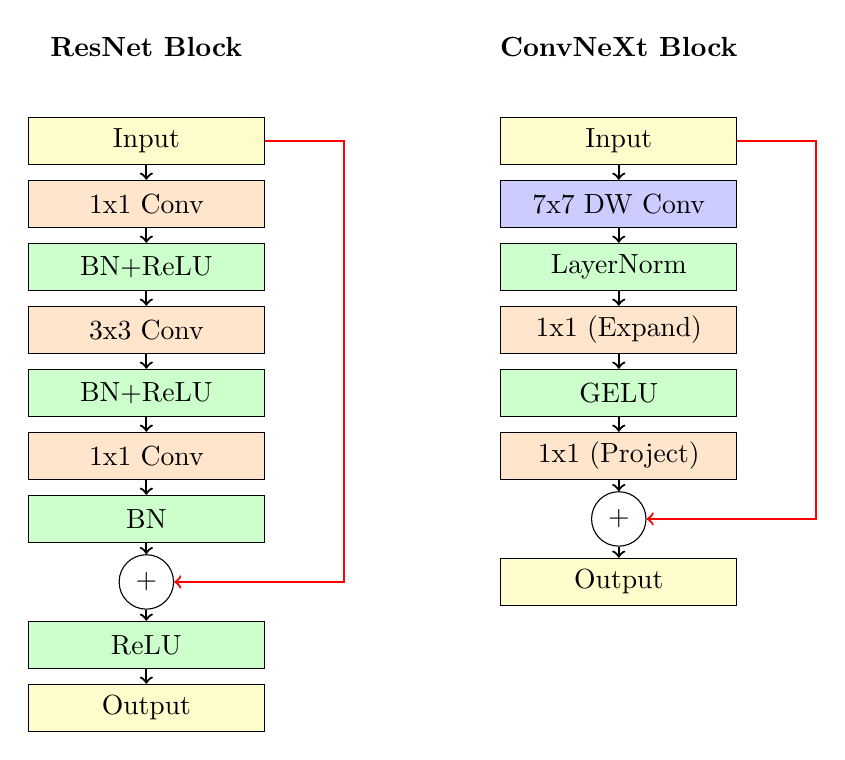
\begin{tikzpicture}[node distance=0.8cm, box/.style={rectangle, draw, minimum width=3cm, minimum height=0.6cm, align=center}]

% ResNet Block
\node[box, fill=yellow!20] (r1) {Input};
\node[box, fill=orange!20, below of=r1] (r2) {1x1 Conv};
\node[box, fill=green!20, below of=r2] (r3) {BN+ReLU};
\node[box, fill=orange!20, below of=r3] (r4) {3x3 Conv};
\node[box, fill=green!20, below of=r4] (r5) {BN+ReLU};
\node[box, fill=orange!20, below of=r5] (r6) {1x1 Conv};
\node[box, fill=green!20, below of=r6] (r7) {BN};
\node[draw, circle, below of=r7, minimum size=0.6cm] (rplus) {+};
\node[box, fill=green!20, below of=rplus] (rrelu) {ReLU};
\node[box, fill=yellow!20, below of=rrelu] (rout) {Output};

\draw[->, thick] (r1) -- (r2);
\draw[->, thick] (r2) -- (r3);
\draw[->, thick] (r3) -- (r4);
\draw[->, thick] (r4) -- (r5);
\draw[->, thick] (r5) -- (r6);
\draw[->, thick] (r6) -- (r7);
\draw[->, thick] (r7) -- (rplus);
\draw[->, thick, red] (r1.east) -- ++(1,0) |- (rplus.east);
\draw[->, thick] (rplus) -- (rrelu);
\draw[->, thick] (rrelu) -- (rout);

\node[above of=r1, node distance=1.2cm, font=\bfseries] {ResNet Block};

% ConvNeXt Block  
\begin{scope}[xshift=6cm]
\node[box, fill=yellow!20] (c1) {Input};
\node[box, fill=blue!20, below of=c1] (c2) {7x7 DW Conv};
\node[box, fill=green!20, below of=c2] (c3) {LayerNorm};
\node[box, fill=orange!20, below of=c3] (c4) {1x1 (Expand)};
\node[box, fill=green!20, below of=c4] (c5) {GELU};
\node[box, fill=orange!20, below of=c5] (c6) {1x1 (Project)};
\node[draw, circle, below of=c6, minimum size=0.6cm] (cplus) {+};
\node[box, fill=yellow!20, below of=cplus] (cout) {Output};

\draw[->, thick] (c1) -- (c2);
\draw[->, thick] (c2) -- (c3);
\draw[->, thick] (c3) -- (c4);
\draw[->, thick] (c4) -- (c5);
\draw[->, thick] (c5) -- (c6);
\draw[->, thick] (c6) -- (cplus);
\draw[->, thick, red] (c1.east) -- ++(1,0) |- (cplus.east);
\draw[->, thick] (cplus) -- (cout);

\node[above of=c1, node distance=1.2cm, font=\bfseries] {ConvNeXt Block};
\end{scope}

\end{tikzpicture}
\caption{Comparison of ResNet and ConvNeXt block architectures}
\end{figure}

\textbf{Key differences:}
\begin{itemize}
    \item ConvNeXt uses inverted bottleneck (expand then compress)
    \item Large depthwise kernel (7x7 vs 3x3)
    \item Fewer normalization/activation layers
    \item LayerNorm instead of BatchNorm
    \item GELU instead of ReLU
\end{itemize}

\section{Part 3: The Modern Training Recipe}

\begin{tcolorbox}[colback=green!5!white, colframe=green!75!black, title=Critical Insight]
The \textit{training recipe} contributes as much to final performance as the architecture itself. Standard ResNet training from 2015 is now obsolete.
\end{tcolorbox}

\subsection{Key Components of Modern Training}

\subsubsection{Optimizer: SGD $\rightarrow$ AdamW}

\textbf{SGD with Momentum (SGDm) - Traditional}
\begin{itemize}
    \item Stable, often generalizes well
    \item Requires careful tuning of LR and momentum
    \item Update rule: $\theta_{t+1} = \theta_t - \eta \nabla L + \mu (\theta_t - \theta_{t-1})$
\end{itemize}

\textbf{Adam - Adaptive Learning Rates}
\begin{itemize}
    \item Adaptive learning rate per parameter
    \item Faster convergence than SGDm
    \item Less sensitive to initial LR
    \item Problem: L2 regularization (weight decay) interacts poorly with adaptive LR
\end{itemize}

\textbf{AdamW - Decoupled Weight Decay}
\begin{itemize}
    \item Fixes Adam by applying weight decay \textit{after} adaptive update
    \item Better generalization than Adam
    \item Easier hyperparameter tuning
    \item \textbf{Modern default for CNNs and Transformers}
\end{itemize}

\subsubsection{Learning Rate Schedule}

\textbf{Step Decay (Legacy):} Abruptly reduce LR at fixed epochs (e.g., 50\%, 75\% of training)

\textbf{Cosine Annealing (Modern):} Smooth decay following cosine curve
\begin{equation}
\eta_t = \eta_{\min} + \frac{1}{2}(\eta_{\max} - \eta_{\min})\left(1 + \cos\left(\frac{t\pi}{T}\right)\right)
\end{equation}

\textbf{Warmup:} Gradually increase LR over first few epochs
\begin{itemize}
    \item Crucial for stability with AdamW and large batch sizes
    \item Prevents early divergence
    \item Typical warmup: 5-10 epochs
\end{itemize}

\subsubsection{Training Duration}

\begin{itemize}
    \item \textbf{Legacy:} 90-120 epochs
    \item \textbf{Modern:} 300+ epochs (requires stronger regularization!)
\end{itemize}

\subsubsection{Advanced Regularization}

\textbf{1. Stochastic Depth (DropPath)}

Instead of dropping individual neurons (Dropout), drop entire residual blocks:
\begin{equation}
H(x) = \text{Bernoulli}(p) \cdot F(x) + x
\end{equation}

\begin{itemize}
    \item Input $x$ bypasses block $F(x)$ via skip connection with probability $(1-p)$
    \item Essential for training very deep networks (100+ layers)
    \item Typical: linear schedule from 0 to 0.1-0.3 across depth
\end{itemize}

\textbf{2. Label Smoothing}

Standard cross-entropy encourages overconfident predictions (target = 1.0). Label smoothing ``softens'' targets:
\begin{equation}
y_{\text{smooth}} = (1-\epsilon)y_{\text{true}} + \frac{\epsilon}{K}
\end{equation}

Example: $[0,1,0] \rightarrow [0.05, 0.9, 0.05]$ with $\epsilon=0.1$

Benefits: Better generalization, improved model calibration

\textbf{3. Advanced Data Augmentation}
\begin{itemize}
    \item AutoAugment: Learned augmentation policies
    \item RandAugment: Simplified automatic augmentation
    \item Mixup \& CutMix: Mix training examples
    \item Random Erasing: Randomly mask image regions
\end{itemize}

\subsection{Legacy vs Modern Recipe Comparison}

\begin{table}[h]
\centering
\begin{tabular}{|l|l|l|}
\hline
\textbf{Component} & \textbf{Legacy (2015)} & \textbf{Modern (2020s)} \\
\hline
Optimizer & SGD + Momentum & AdamW \\
LR Schedule & Step Decay & Cosine + Warmup \\
Epochs & 90-120 & 300+ \\
Augmentation & Flip + Crop & AutoAugment + Erasing \\
Regularization & Dropout & Stochastic Depth + Label Smooth \\
Activation & ReLU & GELU \\
Normalization & BatchNorm & LayerNorm \\
\hline
\end{tabular}
\caption{Evolution of training recipes}
\end{table}

\section{Part 4: Code Implementation and Experiments}

\subsection{Overview of the Playground Code}

The provided code implements a comprehensive experimental framework to demonstrate:

\begin{enumerate}
    \item \textbf{Scaling Experiments:} Compare width-only, depth-only, and compound scaling
    \item \textbf{Modernization Experiments:} Isolate the impact of architecture vs training recipe
\end{enumerate}

\subsection{Architecture: ScalableNet}

The \texttt{ScalableNet} class is a flexible architecture that can host different block types:

\begin{lstlisting}[language=Python, caption=ScalableNet Architecture]
class ScalableNet(nn.Module):
    """
    Flexible CNN supporting different block types and scaling.
    
    Args:
        block_type: StandardBottleneck, MBConvBlock, or ModernizedBlock
        width_mult: Channel multiplier (default 1.0)
        depth_mult: Depth multiplier (default 1.0)
    """
    def __init__(self, block_type, num_classes=100, 
                 width_mult=1.0, depth_mult=1.0):
        super(ScalableNet, self).__init__()
        
        # Base configuration (can be scaled)
        base_channels = [64, 128, 256]
        base_repeats = [2, 3, 2]
        
        # Apply scaling
        channels = [int(c * width_mult) for c in base_channels]
        repeats = [int(math.ceil(r * depth_mult)) 
                   for r in base_repeats]
        
        # Build: Stem -> Stages -> Head
        self.stem = self._make_stem(channels[0])
        self.stages = self._make_stages(channels, repeats)
        self.head = self._make_head(channels[-1], num_classes)
\end{lstlisting}

\subsection{Block Types}

\subsubsection{StandardBottleneck (Legacy ResNet)}

\begin{lstlisting}[language=Python, caption=ResNet Bottleneck Block]
class StandardBottleneck(nn.Module):
    """
    Classic ResNet bottleneck: Compress -> Spatial -> Expand
    Uses BatchNorm and ReLU (legacy design)
    """
    expansion = 4  # Output channels = planes * 4
    
    def __init__(self, in_planes, planes, stride=1):
        super().__init__()
        # 1. Compress: 1x1 conv reduces channels
        self.conv1 = nn.Conv2d(in_planes, planes, 
                               kernel_size=1, bias=False)
        self.bn1 = nn.BatchNorm2d(planes)
        
        # 2. Spatial processing: 3x3 conv
        self.conv2 = nn.Conv2d(planes, planes, kernel_size=3,
                               stride=stride, padding=1, 
                               bias=False)
        self.bn2 = nn.BatchNorm2d(planes)
        
        # 3. Expand: 1x1 conv increases channels
        self.conv3 = nn.Conv2d(planes, self.expansion*planes,
                               kernel_size=1, bias=False)
        self.bn3 = nn.BatchNorm2d(self.expansion*planes)
        
        # Shortcut connection (identity or projection)
        self.shortcut = self._make_shortcut(in_planes, 
                                             planes, stride)
    
    def forward(self, x):
        # Main path: Conv-BN-ReLU pattern
        out = torch.relu(self.bn1(self.conv1(x)))
        out = torch.relu(self.bn2(self.conv2(out)))
        out = self.bn3(self.conv3(out))
        
        # Residual connection
        out += self.shortcut(x)
        out = torch.relu(out)  # ReLU after addition
        return out
\end{lstlisting}

\subsubsection{MBConvBlock (Efficiency-Focused)}

\begin{lstlisting}[language=Python, caption=MobileNet-style Inverted Residual]
class MBConvBlock(nn.Module):
    """
    Inverted residual block: Expand -> DWConv -> Project
    More efficient than standard bottleneck
    """
    expansion = 1
    
    def __init__(self, in_planes, out_planes, 
                 stride=1, expansion_ratio=4):
        super().__init__()
        hidden_dim = int(in_planes * expansion_ratio)
        self.use_res = (stride == 1 and 
                        in_planes == out_planes)
        
        layers = []
        # 1. Expansion: 1x1 conv increases channels
        if expansion_ratio != 1:
            layers.extend([
                nn.Conv2d(in_planes, hidden_dim, 1, bias=False),
                nn.BatchNorm2d(hidden_dim),
                nn.SiLU(inplace=True)  # Swish activation
            ])
        
        # 2. Depthwise Conv: Spatial processing
        #    Each channel processed independently (efficient!)
        layers.extend([
            nn.Conv2d(hidden_dim, hidden_dim, 3, stride, 1,
                      groups=hidden_dim,  # Key: depthwise
                      bias=False),
            nn.BatchNorm2d(hidden_dim),
            nn.SiLU(inplace=True)
        ])
        
        # 3. Projection: 1x1 conv reduces channels
        #    Linear bottleneck (no activation)
        layers.extend([
            nn.Conv2d(hidden_dim, out_planes, 1, bias=False),
            nn.BatchNorm2d(out_planes)
        ])
        
        self.conv = nn.Sequential(*layers)
    
    def forward(self, x):
        if self.use_res:
            return x + self.conv(x)  # Residual
        return self.conv(x)
\end{lstlisting}

\subsubsection{ModernizedBlock (ConvNeXt-Style)}

\begin{lstlisting}[language=Python, caption=ConvNeXt Block]
class ModernizedBlock(nn.Module):
    """
    Modernized ConvNeXt-style block
    Key features:
    - Large depthwise kernel (5x5 or 7x7)
    - LayerNorm instead of BatchNorm
    - GELU activation
    - Inverted bottleneck MLP
    """
    expansion = 1
    
    def __init__(self, dim, stride=1, expansion_ratio=4):
        super().__init__()
        
        # Handle spatial downsampling in separate path
        self.downsample = None
        if stride != 1:
            self.downsample = nn.AvgPool2d(stride, stride)
        
        # 1. Large kernel depthwise conv (5x5)
        #    Larger than traditional 3x3!
        self.dwconv = nn.Conv2d(dim, dim, kernel_size=5,
                                padding=2, groups=dim, 
                                stride=stride)
        
        # 2. Channel-wise LayerNorm (not BatchNorm!)
        self.norm = LayerNorm(dim, eps=1e-6, 
                              data_format="channels_last")
        
        # 3. Inverted bottleneck MLP
        hidden_dim = expansion_ratio * dim
        self.pwconv1 = nn.Linear(dim, hidden_dim)
        self.act = nn.GELU()  # Not ReLU!
        self.pwconv2 = nn.Linear(hidden_dim, dim)
    
    def forward(self, x):
        input = x
        if self.downsample is not None:
            input = self.downsample(x)
        
        # Apply depthwise conv
        x = self.dwconv(x)
        
        # LayerNorm + MLP (requires HWC format)
        x = x.permute(0, 2, 3, 1)  # NCHW -> NHWC
        x = self.norm(x)
        x = self.pwconv1(x)
        x = self.act(x)
        x = self.pwconv2(x)
        x = x.permute(0, 3, 1, 2)  # NHWC -> NCHW
        
        # Residual connection
        return input + x
\end{lstlisting}

\subsection{Training Recipe Implementation}

\begin{lstlisting}[language=Python, caption=Training Configuration]
def get_training_components(model, config_type):
    """
    Configure optimizer, scheduler, and loss based on recipe
    
    Args:
        config_type: 'legacy' or 'modern'
    
    Returns:
        optimizer, scheduler, criterion, num_epochs
    """
    if config_type == 'legacy':
        # --- Legacy Recipe (circa 2015) ---
        # SGD with momentum, standard settings
        optimizer = optim.SGD(model.parameters(), 
                              lr=0.1,           # High initial LR
                              momentum=0.9,
                              weight_decay=1e-4)
        
        # Step decay: reduce LR at 50% and 75% of training
        milestones = [int(EPOCHS * 0.5), int(EPOCHS * 0.75)]
        scheduler = optim.lr_scheduler.MultiStepLR(
            optimizer, milestones=milestones, gamma=0.1)
        
        # Standard cross-entropy
        criterion = nn.CrossEntropyLoss()
        epochs = 90  # Shorter training
        
    elif config_type == 'modern':
        # --- Modern Recipe (circa 2020+) ---
        # AdamW with decoupled weight decay
        optimizer = optim.AdamW(model.parameters(),
                                lr=1e-3,        # Lower initial LR
                                weight_decay=0.05)  # Stronger decay
        
        # Cosine annealing: smooth LR decay
        scheduler = CosineAnnealingLR(optimizer, T_max=EPOCHS)
        
        # Label smoothing for better calibration
        criterion = nn.CrossEntropyLoss(label_smoothing=0.1)
        epochs = 300  # Longer training!
    
    return optimizer, scheduler, criterion, epochs
\end{lstlisting}

\subsection{Experiment 1: Scaling}

This experiment demonstrates the importance of balanced scaling:

\begin{lstlisting}[language=Python, caption=Scaling Experiment]
def experiment_scaling():
    """
    Compare different scaling strategies on MBConvBlock
    
    Configurations tested:
    1. Baseline (W=1.0, D=1.0)
    2. Width-only (W=1.4, D=1.0) 
    3. Depth-only (W=1.0, D=1.4)
    4. Compound (W=1.2, D=1.2) - balanced
    """
    configs = {
        "Baseline": {"width_mult": 1.0, "depth_mult": 1.0},
        "Width Only": {"width_mult": 1.4, "depth_mult": 1.0},
        "Depth Only": {"width_mult": 1.0, "depth_mult": 1.4},
        "Compound": {"width_mult": 1.2, "depth_mult": 1.2},
    }
    
    # Use modern recipe for all (fair comparison)
    trainloader, testloader = get_dataloaders(
        use_modern_aug=True)
    
    results = {}
    for name, config in configs.items():
        print(f"\nTraining: {name}")
        
        # Create model with scaling
        model = ScalableNet(MBConvBlock, **config)
        params = count_parameters(model)
        print(f"Parameters: {params/1e6:.2f}M")
        
        # Train with modern recipe
        acc = run_training(model, trainloader, testloader,
                          config_type='modern')
        results[name] = (acc, params)
    
    # Expected observation:
    # Compound scaling achieves best accuracy-per-parameter
    # Single-axis scaling wastes capacity
\end{lstlisting}

\begin{tcolorbox}[colback=blue!5!white, colframe=blue!75!black, title=Expected Results]
\textbf{Typical outcomes:}
\begin{itemize}
    \item \textbf{Width-only:} Moderate gain, high parameter cost
    \item \textbf{Depth-only:} Small gain, optimization challenges
    \item \textbf{Compound:} Best accuracy per parameter, balanced growth
\end{itemize}

The compound scaling curve should stay efficient longer than single-axis approaches.
\end{tcolorbox}

\subsection{Experiment 2: Modernization}

This experiment isolates the contributions of architecture vs training recipe:

\begin{lstlisting}[language=Python, caption=Modernization Experiment]
def experiment_modernization():
    """
    Isolate the impact of architecture vs training recipe
    
    Three setups:
    1. Legacy Arch + Legacy Recipe (baseline)
    2. Legacy Arch + Modern Recipe (recipe impact)
    3. Modern Arch + Modern Recipe (full modernization)
    """
    
    # Setup 1: Legacy + Legacy (circa 2015)
    print("\n=== Legacy Architecture + Legacy Recipe ===")
    trainloader_legacy, testloader = get_dataloaders(
        use_modern_aug=False)  # Basic augmentation
    
    model_legacy = ScalableNet(StandardBottleneck,
                               width_mult=1.0, 
                               depth_mult=1.0)
    params_legacy = count_parameters(model_legacy)
    print(f"Parameters: {params_legacy/1e6:.2f}M")
    
    acc_legacy = run_training(model_legacy, 
                              trainloader_legacy,
                              testloader,
                              config_type='legacy')
    
    # Setup 2: Legacy + Modern Recipe
    print("\n=== Legacy Architecture + Modern Recipe ===")
    trainloader_modern, testloader = get_dataloaders(
        use_modern_aug=True)  # Strong augmentation
    
    model_legacy_modern = ScalableNet(StandardBottleneck,
                                      width_mult=1.0,
                                      depth_mult=1.0)
    
    acc_recipe_impact = run_training(model_legacy_modern,
                                     trainloader_modern,
                                     testloader,
                                     config_type='modern')
    
    # Setup 3: Modern Architecture + Modern Recipe
    print("\n=== Modern Architecture + Modern Recipe ===")
    model_modern = ScalableNet(ModernizedBlock,
                               width_mult=1.5,  # Adjusted for 
                               depth_mult=1.0)  # param count
    params_modern = count_parameters(model_modern)
    print(f"Parameters: {params_modern/1e6:.2f}M")
    
    acc_modern = run_training(model_modern,
                             trainloader_modern,
                             testloader,
                             config_type='modern')
    
    # Analysis
    print("\n=== Results ===")
    print(f"1. Legacy + Legacy: {acc_legacy:.2f}%")
    print(f"2. Legacy + Modern Recipe: {acc_recipe_impact:.2f}%")
    print(f"3. Modern + Modern: {acc_modern:.2f}%")
    print(f"\nRecipe contribution: "
          f"+{acc_recipe_impact - acc_legacy:.2f}%")
    print(f"Architecture contribution: "
          f"+{acc_modern - acc_recipe_impact:.2f}%")
\end{lstlisting}

\begin{tcolorbox}[colback=green!5!white, colframe=green!75!black, title=Key Insight from Experiment 2]
\textbf{Expected finding:} Both the modern recipe AND the modernized architecture contribute significantly. The recipe change often provides a larger boost than architectural changes alone!

This demonstrates that training methodology is as important as network design.
\end{tcolorbox}

\section{Practical Considerations}

\subsection{When to Use Each Approach}

\begin{table}[h]
\centering
\begin{tabular}{|l|p{8cm}|}
\hline
\textbf{Scenario} & \textbf{Recommendation} \\
\hline
Embedded/Mobile & MBConvBlock with width scaling only \\
Cloud/Server & Compound scaling (EfficientNet-style) \\
Limited data & Modern recipe crucial; avoid over-scaling \\
Large datasets & Both architecture \& scaling improvements pay off \\
Need speed & Width scaling + modern optimizations (FusedMBConv) \\
\hline
\end{tabular}
\end{table}

\subsection{Common Pitfalls}

\begin{enumerate}
    \item \textbf{Ignoring the recipe:} Using modern architectures with legacy training
    \item \textbf{Over-regularization:} Too much augmentation/dropout for small datasets
    \item \textbf{BatchNorm issues:} Small batch sizes make BN unstable (use GroupNorm or LayerNorm)
    \item \textbf{FLOPs $\neq$ Latency:} Always profile on target hardware
    \item \textbf{Memory-bound ops:} Large models may be bandwidth-limited, not compute-limited
\end{enumerate}

\section{Summary and Key Takeaways}

\subsection{Core Principles Synthesized}

The evolution from ResNet (2015) to ConvNeXt (2022) and beyond crystallizes fundamental principles for modern deep learning:

\begin{enumerate}
    \item \textbf{Balanced Scaling is Necessary:} Single-axis scaling wastes compute. Compound scaling provides a principled, efficient growth path that respects the interdependence of depth, width, and resolution.
    
    \item \textbf{Recipe is Paramount:} Modern training systems (AdamW, cosine schedules, 300+ epochs, strong regularization) contribute as much or more to performance than architectural changes. Always modernize training before abandoning an architecture.
    
    \item \textbf{Architectural Convergence:} CNNs and Transformers are converging. The most effective designs borrow ideas across paradigms: large kernels (expanding ERF), inverted bottlenecks (efficiency), LayerNorm (stability), GELU (smooth gradients).
    
    \item \textbf{Hardware Co-Design:} Theoretical FLOPs $\neq$ practical latency. Design decisions must account for memory bandwidth, cache efficiency, and accelerator architecture. InceptionNeXt exemplifies hardware-aware design.
    
    \item \textbf{Holistic System Design:} Performance emerges from the tight coupling of architecture, training recipe, data augmentation, and regularization. No single component determines success---all must evolve together.
\end{enumerate}

\subsection{The Evolution Timeline}

\begin{center}
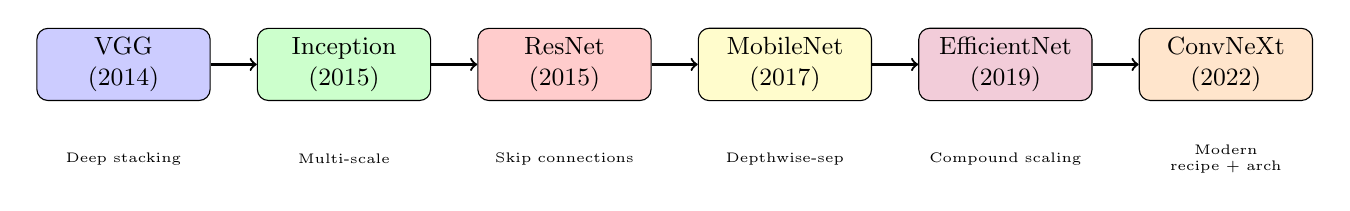
\begin{tikzpicture}[node distance=2cm, box/.style={rectangle, draw, rounded corners, minimum width=2.2cm, minimum height=0.8cm, align=center, font=\small}]

\node[box, fill=blue!20] (vgg) {VGG\\(2014)};
\node[box, right of=vgg, node distance=2.8cm, fill=green!20] (inception) {Inception\\(2015)};
\node[box, right of=inception, node distance=2.8cm, fill=red!20] (resnet) {ResNet\\(2015)};
\node[box, right of=resnet, node distance=2.8cm, fill=yellow!20] (mobile) {MobileNet\\(2017)};
\node[box, right of=mobile, node distance=2.8cm, fill=purple!20] (efficient) {EfficientNet\\(2019)};
\node[box, right of=efficient, node distance=2.8cm, fill=orange!20] (convnext) {ConvNeXt\\(2022)};

\draw[->, thick] (vgg) -- (inception);
\draw[->, thick] (inception) -- (resnet);
\draw[->, thick] (resnet) -- (mobile);
\draw[->, thick] (mobile) -- (efficient);
\draw[->, thick] (efficient) -- (convnext);

\node[below of=vgg, node distance=1.2cm, font=\tiny, text width=2.2cm, align=center] {Deep stacking};
\node[below of=inception, node distance=1.2cm, font=\tiny, text width=2.2cm, align=center] {Multi-scale};
\node[below of=resnet, node distance=1.2cm, font=\tiny, text width=2.2cm, align=center] {Skip connections};
\node[below of=mobile, node distance=1.2cm, font=\tiny, text width=2.2cm, align=center] {Depthwise-sep};
\node[below of=efficient, node distance=1.2cm, font=\tiny, text width=2.2cm, align=center] {Compound scaling};
\node[below of=convnext, node distance=1.2cm, font=\tiny, text width=2.2cm, align=center] {Modern recipe + arch};

\end{tikzpicture}
\end{center}

\subsection{When to Use What}

\begin{table}[h]
\centering
\small
\begin{tabular}{|l|l|p{6cm}|}
\hline
\textbf{Scenario} & \textbf{Architecture} & \textbf{Rationale} \\
\hline
Edge/Mobile deployment & MobileNetV3, EfficientNet-Lite & Low latency, small memory, optimized for TFLite/CoreML \\
\hline
Limited training data & ConvNeXt, ResNet with modern recipe & Strong inductive biases, data-efficient \\
\hline
Large-scale training & Hybrid (CoAtNet), ViT & Best scaling properties, SOTA performance \\
\hline
High-resolution inputs & CNN-based (ConvNeXt, InceptionNeXt) & Efficient spatial processing, manageable memory \\
\hline
Need interpretability & Pure CNN with attention maps & Clear spatial hierarchies, visualizable features \\
\hline
Zero-shot generalization & Foundation models (DINOv2, CLIP) & Pre-trained on massive diverse data \\
\hline
\end{tabular}
\caption{Architecture selection guide}
\end{table}

\subsection{Common Pitfalls and How to Avoid Them}

\begin{enumerate}
    \item \textbf{Using outdated training recipes}
    \begin{itemize}
        \item Symptom: Modern architecture performs poorly
        \item Solution: Update to AdamW, cosine schedule, 300+ epochs, strong augmentation
    \end{itemize}
    
    \item \textbf{Over-regularization on small datasets}
    \begin{itemize}
        \item Symptom: Large train-val gap, underfitting
        \item Solution: Reduce stochastic depth probability, weaken augmentation, use fewer epochs
    \end{itemize}
    
    \item \textbf{BatchNorm with small batches}
    \begin{itemize}
        \item Symptom: Training instability, poor test performance
        \item Solution: Switch to LayerNorm or GroupNorm, or increase batch size
    \end{itemize}
    
    \item \textbf{Ignoring hardware constraints}
    \begin{itemize}
        \item Symptom: Model is fast in FLOPs but slow in practice
        \item Solution: Profile on target hardware, optimize memory-bound operations
    \end{itemize}
    
    \item \textbf{Single-axis scaling}
    \begin{itemize}
        \item Symptom: Performance saturates despite adding compute
        \item Solution: Use compound scaling, balance all three dimensions
    \end{itemize}
    
    \item \textbf{Not using warmup with AdamW}
    \begin{itemize}
        \item Symptom: Training diverges or is unstable early on
        \item Solution: Add 5-10 epoch linear warmup at the start
    \end{itemize}
\end{enumerate}

\subsection{Final Reflection}

\begin{tcolorbox}[colback=blue!5!white, colframe=blue!75!black, title=The Deeper Lesson]
The journey from VGG to ConvNeXt teaches us that progress in deep learning is not about finding a single ``winning architecture.'' Instead, it emerges from the \textit{virtuous cycle} of:

\begin{center}
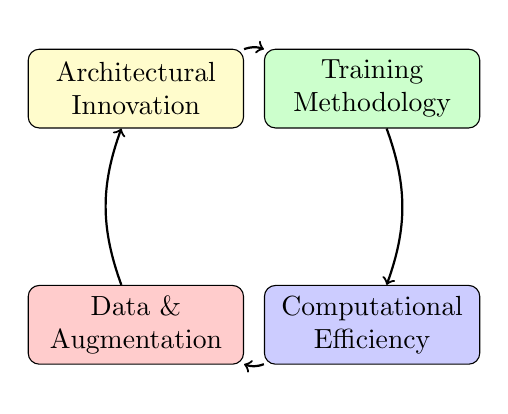
\begin{tikzpicture}[node distance=3cm, auto, box/.style={rectangle, draw, rounded corners, text width=2.5cm, align=center, minimum height=1cm}]

\node[box, fill=yellow!20] (arch) {Architectural\\Innovation};
\node[box, right of=arch, fill=green!20] (recipe) {Training\\Methodology};
\node[box, below of=recipe, fill=blue!20] (hardware) {Computational\\Efficiency};
\node[box, left of=hardware, fill=red!20] (data) {Data \&\\Augmentation};

\draw[->, thick, bend left=20] (arch) to node {} (recipe);
\draw[->, thick, bend left=20] (recipe) to node {} (hardware);
\draw[->, thick, bend left=20] (hardware) to node {} (data);
\draw[->, thick, bend left=20] (data) to node {} (arch);

\end{tikzpicture}
\end{center}

Each component enables and constrains the others. Modern CNNs succeed not because convolution is ``better'' than attention, but because we've learned to design the entire system holistically---from architecture to optimizer to augmentation to hardware deployment.

The future belongs to practitioners who understand this interconnectedness and can navigate trade-offs across the full stack of deep learning systems.
\end{tcolorbox}

\section{Exercises and Discussion}

\subsection{Conceptual Questions}

\begin{enumerate}
    \item Why does the compound scaling constraint $\alpha \beta^2 \gamma^2 \approx 2$ make sense given the FLOPs formula?
    
    \item Explain why label smoothing improves generalization. What problem does it address?
    
    \item Why is LayerNorm preferred over BatchNorm in modern architectures?
    
    \item How does stochastic depth differ from dropout? When is each more appropriate?
    
    \item \textbf{The ``Rule Breaking'' Question:} We established that 3x3 kernels are optimal (VGG), that BatchNorm is essential (ResNet), and that bottlenecks should compress-then-expand (ResNet). ConvNeXt uses 7x7 kernels, LayerNorm, and inverted bottlenecks. Are the earlier principles wrong?
    
    \textit{Answer guide:} No---they were correct for their context. Discuss how:
    \begin{itemize}
        \item Hardware evolved (better memory bandwidth, Tensor Cores)
        \item Training methods changed (AdamW enables larger kernels, 300 epochs allows more parameters)
        \item Requirements shifted (need for global context to compete with ViTs)
        \item Principles remain (need for normalization, activation, receptive field), but optimal implementations evolved
    \end{itemize}
\end{enumerate}

\subsection{The Pattern of ``Rule Evolution'' in Deep Learning}

This isn't the first time ``established rules'' have evolved. Understanding this pattern helps us think critically about current best practices:

\begin{table}[h]
\centering
\small
\begin{tabular}{|l|l|l|l|}
\hline
\textbf{Era} & \textbf{``Rule''} & \textbf{Later ``Broken'' By} & \textbf{Why It Changed} \\
\hline
2012 & 
\begin{tabular}[t]{@{}l@{}}
``Deep learning \\
needs pretraining''
\end{tabular} & 
\begin{tabular}[t]{@{}l@{}}
AlexNet (2012)\\
trained from scratch
\end{tabular} & 
\begin{tabular}[t]{@{}l@{}}
ReLU + Dropout enabled\\
training without pretraining
\end{tabular} \\
\hline
2014 & 
\begin{tabular}[t]{@{}l@{}}
``Small kernels\\
(3x3) are best''
\end{tabular} & 
\begin{tabular}[t]{@{}l@{}}
ConvNeXt (2022)\\
uses 7x7 kernels
\end{tabular} & 
\begin{tabular}[t]{@{}l@{}}
Modern training enables\\
larger kernels without overfitting
\end{tabular} \\
\hline
2015 & 
\begin{tabular}[t]{@{}l@{}}
``BatchNorm is\\
essential''
\end{tabular} & 
\begin{tabular}[t]{@{}l@{}}
Transformers use\\
LayerNorm
\end{tabular} & 
\begin{tabular}[t]{@{}l@{}}
Batch-size independence\\
more important for flexibility
\end{tabular} \\
\hline
2017 & 
\begin{tabular}[t]{@{}l@{}}
``Attention is\\
too expensive''
\end{tabular} & 
\begin{tabular}[t]{@{}l@{}}
ViT (2020) uses\\
pure attention
\end{tabular} & 
\begin{tabular}[t]{@{}l@{}}
Hardware improved,\\
showed attention scales well
\end{tabular} \\
\hline
2020 & 
\begin{tabular}[t]{@{}l@{}}
``CNNs can't match\\
Transformers''
\end{tabular} & 
\begin{tabular}[t]{@{}l@{}}
ConvNeXt (2022)\\
matches ViTs
\end{tabular} & 
\begin{tabular}[t]{@{}l@{}}
Recipe + architecture\\
modernization closes gap
\end{tabular} \\
\hline
\end{tabular}
\caption{The recurring pattern: ``rules'' evolve as context changes}
\end{table}

\begin{tcolorbox}[colback=purple!5!white, colframe=purple!75!black, title=Critical Thinking Framework]
When encountering ``established rules'' in deep learning, always ask:

\begin{enumerate}
    \item \textbf{What constraints was this optimized for?} (Hardware? Data? Compute budget?)
    \item \textbf{What problem was it solving?} (Vanishing gradients? Overfitting? Speed?)
    \item \textbf{Have those constraints changed?} (New hardware? More data? Better optimizers?)
    \item \textbf{What's the underlying principle?} (Not ``use BatchNorm'' but ``normalize activations'')
    \item \textbf{Are there now better ways to achieve that principle?}
\end{enumerate}

This prevents dogmatic thinking and enables genuine innovation.
\end{tcolorbox}

\subsection{Design Exercise: Context-Aware Architecture Selection}

Given the following scenarios, justify your architectural choices by analyzing the context:

\textbf{Scenario 1:} Training a model for deployment on smartphones with 4GB RAM, 100ms latency budget, dataset of 50K images.

\textit{Analysis framework:}
\begin{itemize}
    \item Constraints: Limited memory, strict latency, small dataset
    \item Appropriate choices: MobileNetV3 (efficient), smaller kernels (memory), strong inductive biases (small data), modern recipe but shorter training (to avoid overfitting)
    \item Inappropriate: Large kernels (memory), pure Transformer (data hungry), 300 epoch training (overfitting risk)
\end{itemize}

\textbf{Scenario 2:} Training on 1M labeled images + 100M unlabeled images, deploying in cloud, accuracy is primary concern.

\textit{Analysis framework:}
\begin{itemize}
    \item Constraints: Abundant data, cloud compute available, optimize for accuracy
    \item Appropriate choices: Hybrid architecture (CoAtNet), SSL pre-training on unlabeled data, large models with compound scaling, 300+ epochs
    \item Trade-offs: Higher latency acceptable for accuracy gains
\end{itemize}

\subsection{Practical Exercise: Budgeted Scaling}

\textbf{Task:} Design a scaled CNN for a specific computational budget.

\textbf{Instructions:}
\begin{enumerate}
    \item Pick a baseline: ResNet-50, ConvNeXt-Tiny, or EfficientNet-Lite0
    \item Choose a target device budget (e.g., 100ms inference, 4GB memory)
    \item Propose a $D/W/R$ scaling plan to meet constraints
    \item Justify your recipe choices (optimizer, schedule, regularization)
    \item Predict failure modes (over-regularization, BN statistics issues, memory-bound operations)
\end{enumerate}

\textbf{Deliverable:} Report with plots/tables showing accuracy vs latency trade-offs.

\subsection{Code Exploration}

\begin{enumerate}
    \item \textbf{Modify the scaling:} Edit \texttt{experiment\_scaling()} to try different $(\alpha, \beta, \gamma)$ values. Can you find better combinations for CIFAR-100?
    
    \item \textbf{Hybrid blocks:} Create a model that uses MBConvBlock in early stages and ModernizedBlock in later stages. Does this improve efficiency?
    
    \item \textbf{Ablation study:} Remove one component from the modern recipe (e.g., no label smoothing) and measure the impact.
    
    \item \textbf{AMP (Automatic Mixed Precision):} Enable mixed precision training and measure speedup. Does it affect accuracy?
\end{enumerate}

\section{Looking Ahead}

\subsection{Topics Deferred to Future Lectures}

\begin{itemize}
    \item \textbf{Encoder-Decoder \& U-Net:} Critical for segmentation, image-to-image tasks, and diffusion models (Next Lecture)
    
    \item \textbf{Vision Transformers (ViTs):} The alternative paradigm using self-attention
    
    \item \textbf{Generative Models:} GANs and Diffusion Models for image synthesis
\end{itemize}

\subsection{Topics Deferred to Computer Vision Course}

\begin{itemize}
    \item \textbf{Object Detection:} R-CNN family, YOLO, SSD, specialized losses
    
    \item \textbf{Image Segmentation:} FCN, Mask R-CNN, spatial resolution preservation
\end{itemize}

\section{Additional Resources}

\subsection{Key Papers}

\begin{enumerate}
    \item EfficientNet: Rethinking Model Scaling for Convolutional Neural Networks (Tan \& Le, 2019)
    \item A ConvNet for the 2020s (Liu et al., 2022) - ConvNeXt
    \item Decoupled Weight Decay Regularization (Loshchilov \& Hutter, 2019) - AdamW
    \item Deep Residual Learning for Image Recognition (He et al., 2016) - ResNet
\end{enumerate}

\subsection{Recommended Experiments}

\begin{enumerate}
    \item Profile different blocks (ResNet, MobileNet, ConvNeXt) on your target hardware
    \item Train a small model from scratch with both legacy and modern recipes
    \item Visualize learned features at different depths
    \item Measure effective receptive field with different kernel sizes
\end{enumerate}

\vspace{1cm}

\begin{tcolorbox}[colback=blue!5!white, colframe=blue!75!black, title=Final Thought]
The journey from VGG to ConvNeXt illustrates a fundamental principle: \textit{progress in deep learning comes from the interplay of architectural innovation, training methodology, and computational efficiency.} Neither architecture nor training recipe alone determines success---both must evolve together.
\end{tcolorbox}

\end{document}